\section{Présentation}
\ifprof
\else
\subsection{Contexte}
L'utilisation du mode vidéo, en haute définition sur les appareils photo réflex et légers, pose aux photographes le problème de la stabilisation de l'image car les vibrations engendrées y sont importantes et visibles. Des stabilisateurs installés à l'intérieur des appareils diminuent l'effet de ces vibrations mais ils restent très insuffisants pour assurer une bonne stabilisation notamment sur des sujets mobiles car ces systèmes ne sont efficaces que pour des temps de pose relativement longs. C'est pour cette raison que des systèmes de stabilisation externes ont été développés avec des supports et accessoires purement mécaniques ou motorisés.

\subsection{Nacelles gyrostabilisées}
Parmi les systèmes de stabilisation externes, les nacelles gyrostabilisées, installées sur une perche portée par les deux mains de l'utilisateur et sur lesquelles se fixe l'appareil photographique présentent l'avantage d'être légères, compactes et d'utilisation facile. Elles permettent de corriger les perturbations dues aux mouvements de l'utilisateur selon trois axes de rotations (figure~\ref{fig:01}). Néanmoins, elles ne permettent pas de réduire les perturbations verticales dues à la marche ou à la course de l'utilisateur.

\begin{figure}[H]
\centering
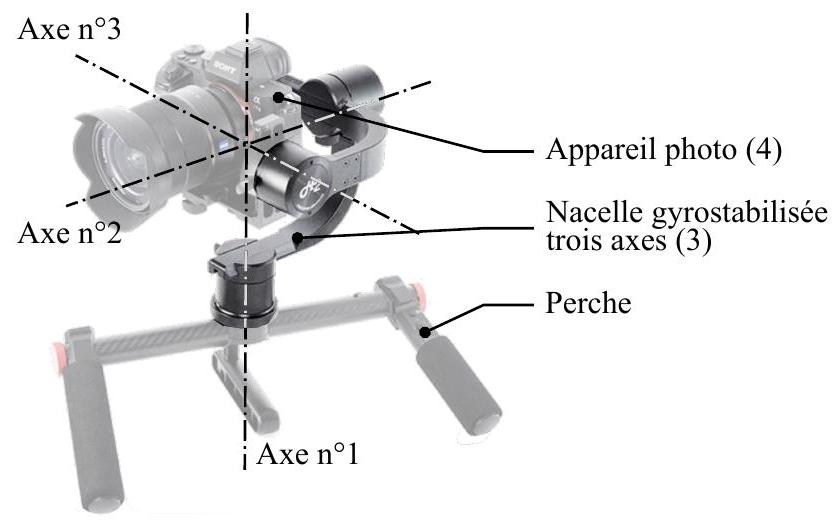
\includegraphics[width=.5\textwidth]{fig_01.jpg}
\caption{\label{fig:01} Nacelle gyrostabilisée}
\end{figure}


\subsection{Stabilisateur vertical}
Pour maitriser les perturbations verticales dues à la marche ou la course des photographes, un constructeur commercialise un stabilisateur vertical à installer entre la perche et la nacelle gyrostabilisée (figure~\ref{fig:02}).

\begin{figure}[H]
\centering
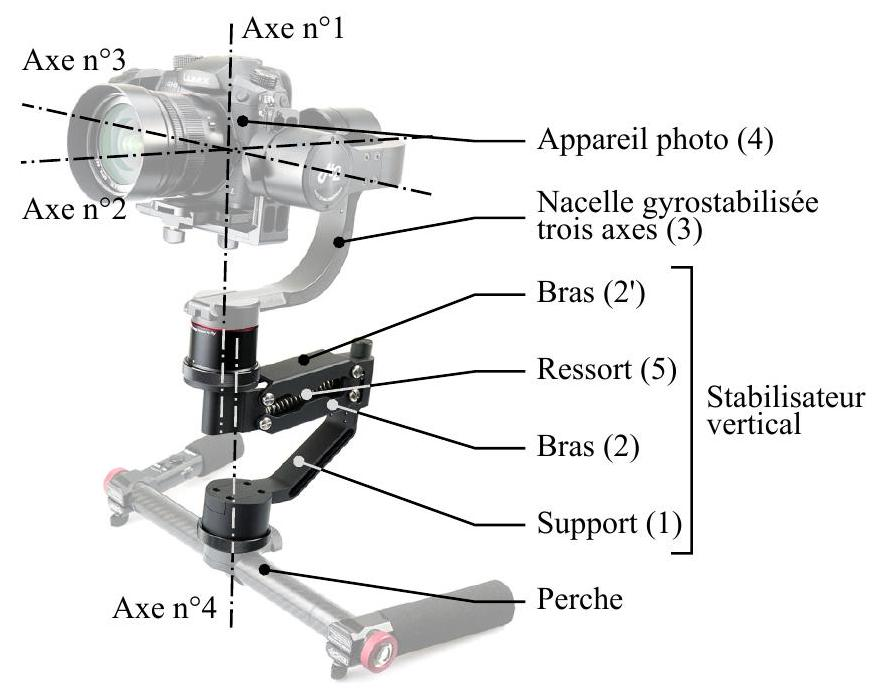
\includegraphics[width=.5\textwidth]{fig_02.jpg}
\caption{\label{fig:02} Nacelle gyrostabilisée avec stabilisateur vertical}
\end{figure}


Une analyse du besoin des photographes a permis de documenter le cahier des charges fonctionnel dont un extrait est donné figure~\ref{fig:A} du document réponse. Le cadre de ce sujet porte plus spécifiquement sur l'évaluation des solutions retenues pour satisfaire les objectifs de maitrise de la position d'un appareil photo à l'équilibre et en mouvement. Le sujet est décomposé en quatre parties :

\begin{itemize}
  \item dans la partie \ref{part:1}, une analyse des mouvements de marche et de course d'un utilisateur est effectuée et les critères chiffrés de l'exigence relative à la position de l'appareil photo en mouvement sont justifiés ;
  \item la partie \ref{part:2} porte sur la vérification du respect de l'exigence relative à la position à l'équilibre de l'appareil photo ;
  \item en partie \ref{part:3}, une étude dynamique met en évidence la nécessité d'ajouter une commande active au système pour assurer le respect de l'exigence relative à la position en mouvement de l'appareil photo ;
  \item la partie \ref{part:4} porte sur la conception de la commande active du système en vue d'assurer la maitrise de la position de l'appareil photo avec le niveau de précision requis par le cahier des charges.
\end{itemize}

\fi

\section{\label{part:1}Analyse du mouvement de l'utilisateur et justification du cahier des charges }

\ifprof
\else
\begin{obj}
Analyser les mouvements de l’utilisateur lorsqu’il marche ou lorsqu’il court et justifier les critères
chiffrés de l’exigence relative à la position de l’appareil photo en mouvement
\end{obj}



Pour réduire les perturbations verticales de l'appareil photo, la solution retenue est de filtrer les mouvements de translation verticale de la perche dont les fréquences sont précisées dans le cahier des charges (\ref{fig:A}). Pour justifier ces performances, on réalise des captures du mouvement vertical d'une perche tenue des deux mains par un utilisateur qui se déplace sur un sol plat.

Cette capture de mouvement est réalisée à partir d'un système optoélectronique dont le principe est le suivant : des caméras projettent une lumière dans le spectre infrarouge et détectent la lumière réfléchie par des marqueurs réfléchissants placés sur l'utilisateur. À partir des focales des caméras, de leur position et de leur orientation, il est possible de reconstruire, à chaque instant, par triangulation, la position spatiale des marqueurs et d'en déduire le mouvement vertical des mains, en retenant la valeur moyenne de la position verticale des deux mains. Les graphes des enregistrements de deux passages, marche et course, sont donnés ainsi que leur analyse spectrale (figure~\ref{fig:03}). Le contenu spectral est estimé en utilisant un enregistrement sur une durée limitée et la relation utilisée permet d'obtenir directement les amplitudes des différentes composantes harmoniques. Le calcul du spectre est réalisé pour un ensemble de fréquences choisi selon une distribution linéaire.


\begin{figure}[H]
\centering
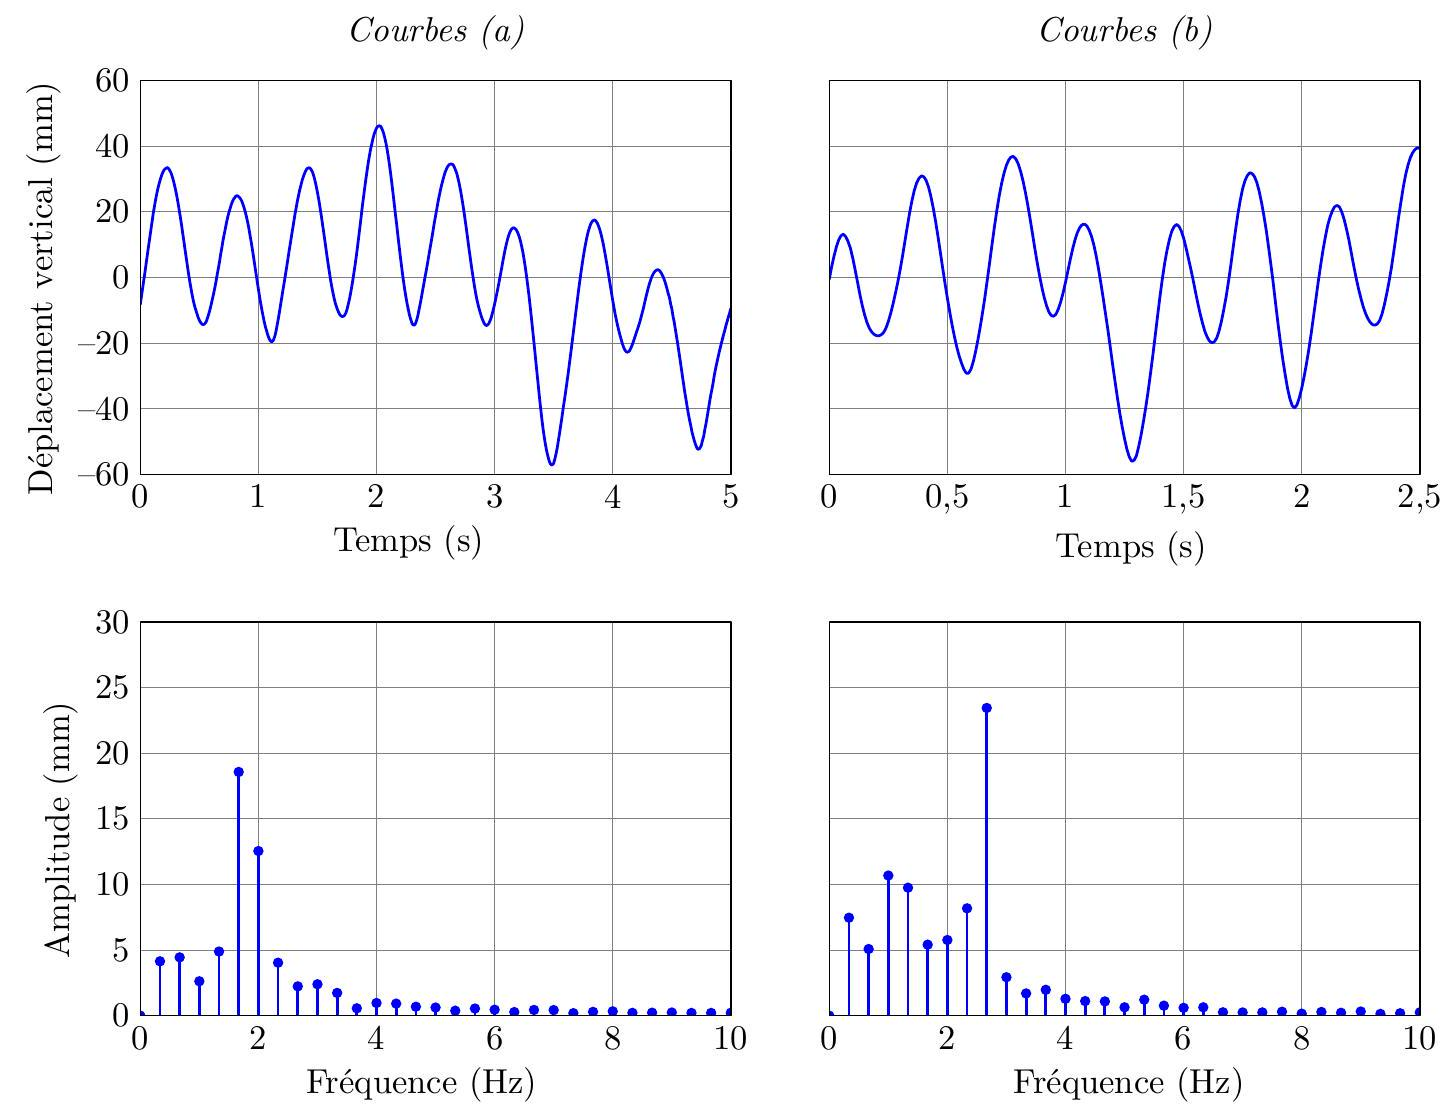
\includegraphics[width=.8\textwidth]{fig_03.jpg}
\caption{\label{fig:03} Représentations temporelle et spectrale du déplacement vertical des mains de l'utilisateur lors de la capture du mouvement}
\end{figure}
\fi
 
%Q 1
\question{\label{q:01} Associer chacune des courbes (a) ou (b) à l'enregistrement du mouvement pendant la marche ou la course de l'utilisateur. Il est conseillé d'analyser les caractéristiques de l'harmonique de plus grande amplitude.}
\ifprof
\begin{corrige}
Sur la courbe de fréquence (a), l’harmonique la plus grande se trouve à une fréquence de $\SI{1,66}{Hz}$.

Sur la courbe de fréquence (b), l’harmonique la plus grande se trouve à une fréquence de $\SI{2,66}{Hz}$.

La fréquence la plus plus basse (a) correspond à la marche. La fréquence la plus haute (b) correspond à la course.

\end{corrige}
\else
\fi

%Q 2. 
\question{\label{q:02} Proposer une méthode de filtrage pour atténuer les perturbations dues à la marche ou à la course de l'utilisateur tout en conservant les mouvements de translation verticale souhaités.}
\ifprof
\begin{corrige}

Pour filtrer les perturbations, il serait possible d'utiliser un filtre coupe-bande, atténuant les fréquences au voisinage de la fréquence de déplacement.
\end{corrige}
\else
\fi
